\documentclass{standalone}
\usepackage{tikz}
\usetikzlibrary{shapes,arrows,positioning,calc,decorations.pathreplacing}

% Define colors
\definecolor{inputblue}{RGB}{173,216,230}
\definecolor{encodergreen}{RGB}{144,238,144}
\definecolor{slicered}{RGB}{240,128,128}
\definecolor{fusionyellow}{RGB}{255,255,224}
\definecolor{poolorange}{RGB}{255,165,0}
\definecolor{taskpurple}{RGB}{186,85,211}
\definecolor{outputblack}{RGB}{50,50,50}

\begin{document}
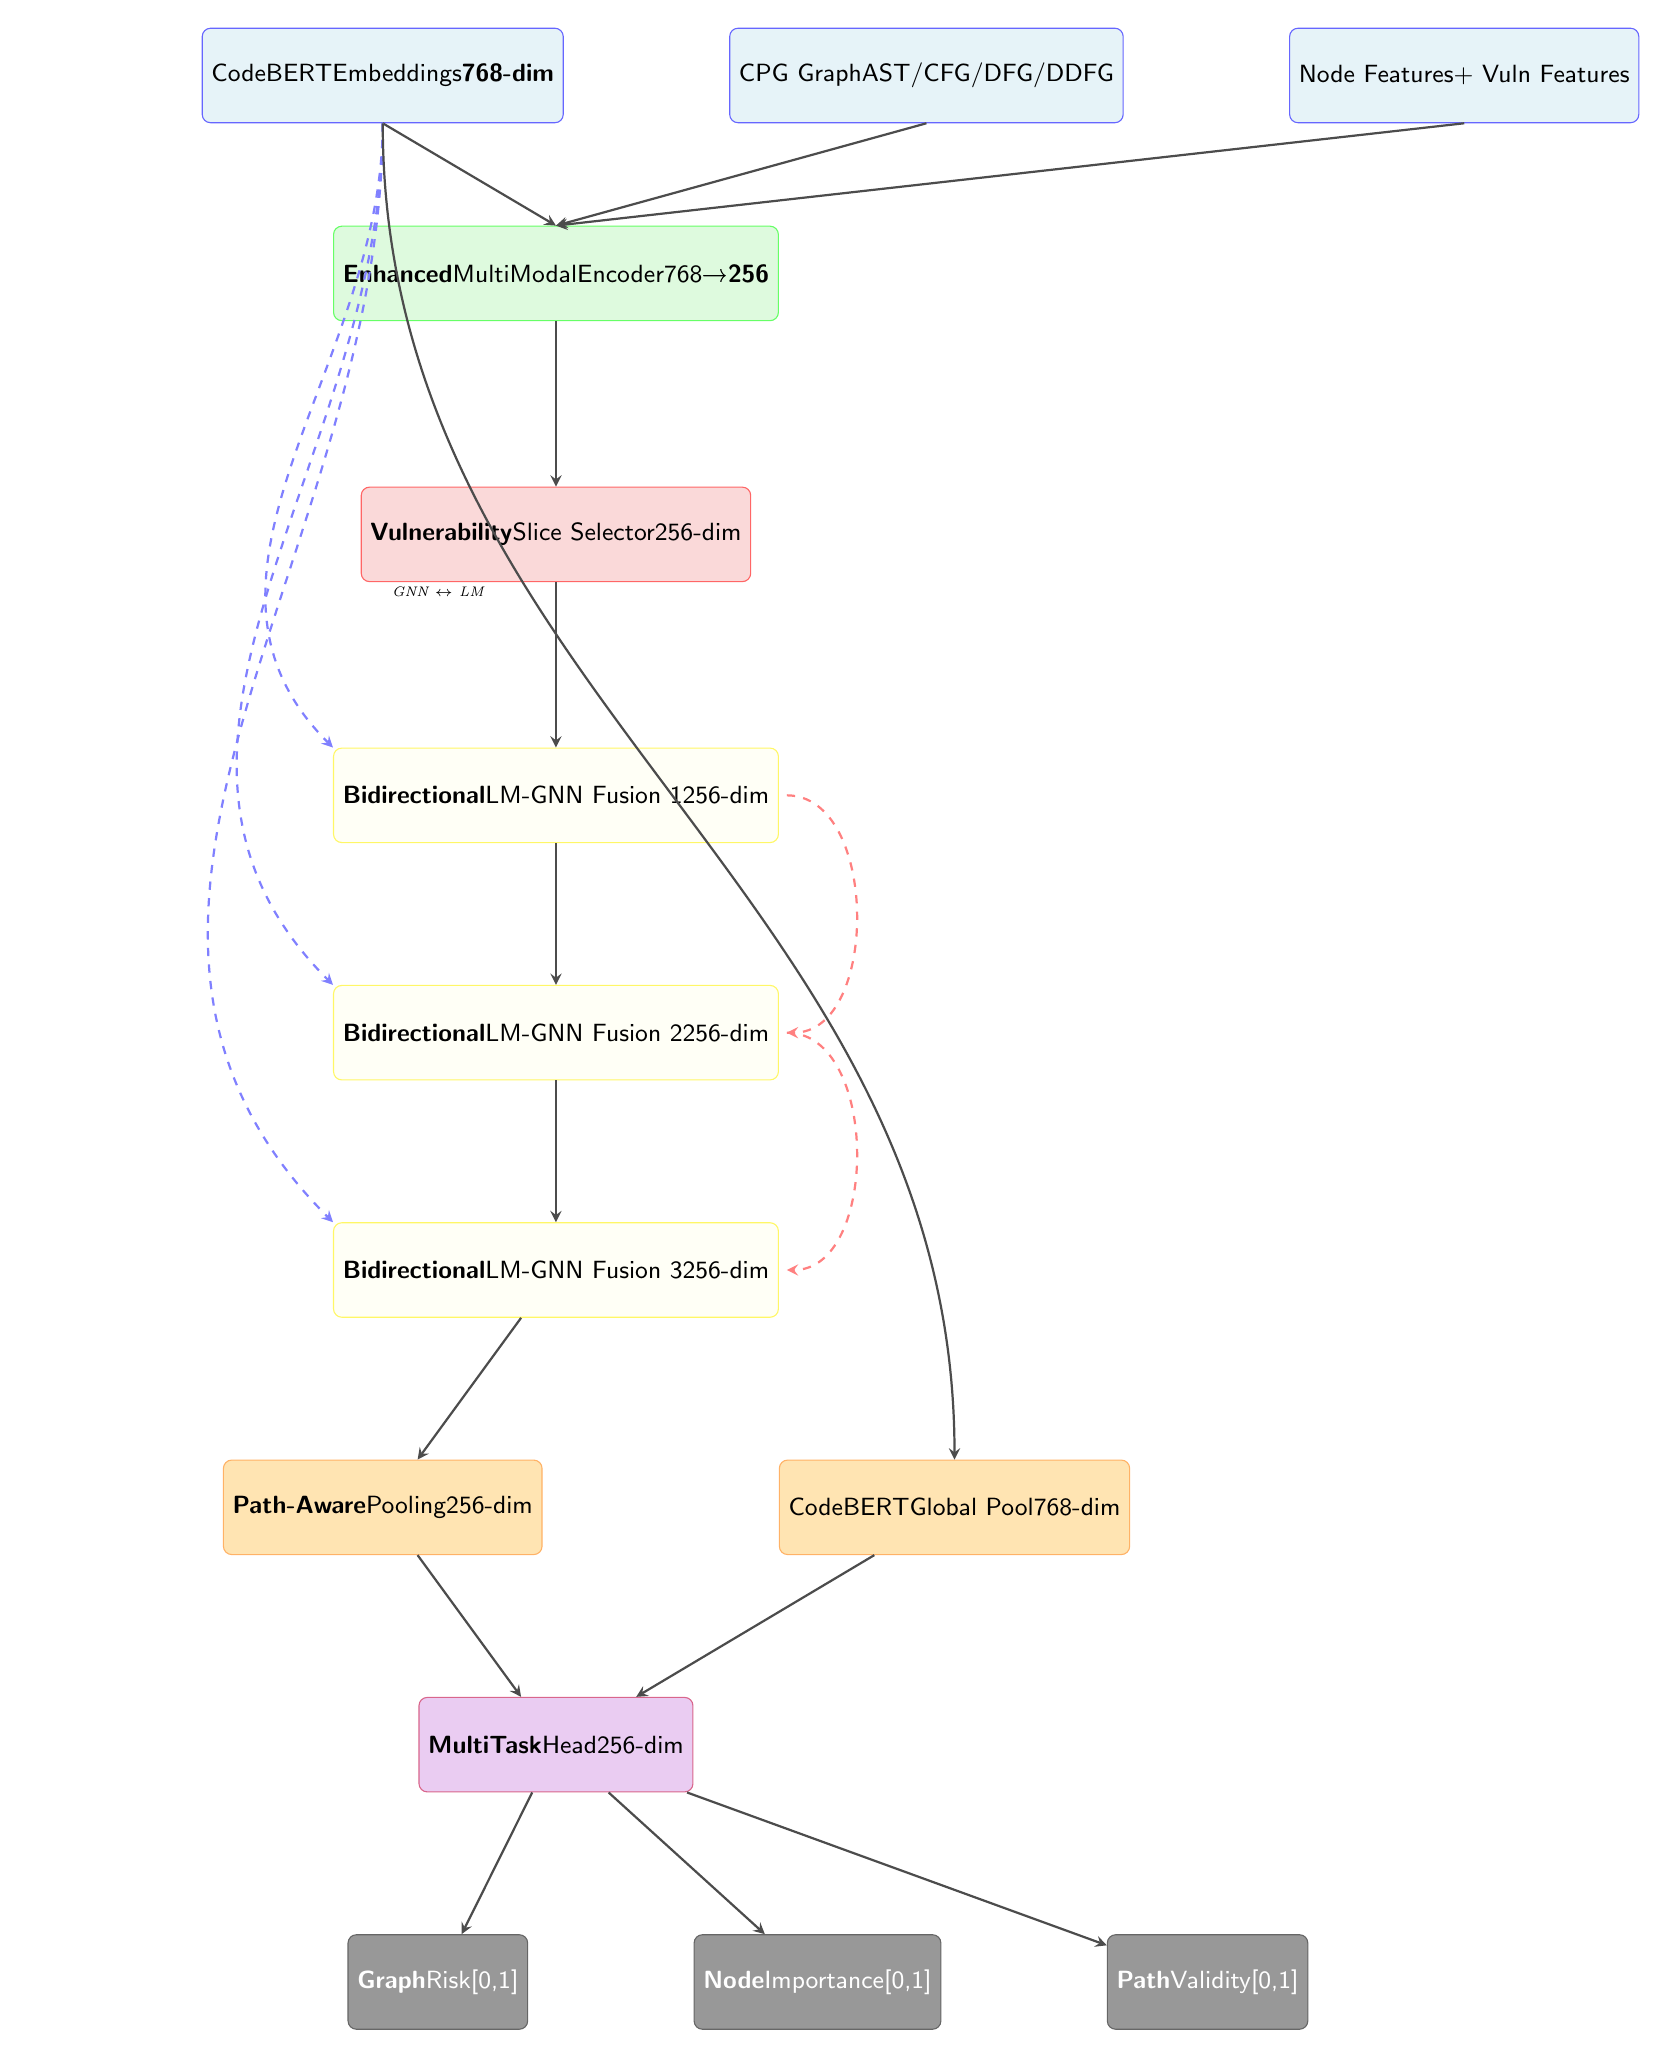
\begin{tikzpicture}[
    node distance=1.8cm,
    every node/.style={font=\small\sffamily},
    input/.style={rectangle, draw=blue!60, fill=inputblue!30, minimum width=2.2cm, minimum height=1.2cm, text centered, rounded corners=3pt},
    encoder/.style={rectangle, draw=green!60, fill=encodergreen!30, minimum width=2.2cm, minimum height=1.2cm, text centered, rounded corners=3pt},
    slice/.style={rectangle, draw=red!60, fill=slicered!30, minimum width=2.2cm, minimum height=1.2cm, text centered, rounded corners=3pt},
    fusion/.style={rectangle, draw=yellow!60, fill=fusionyellow!30, minimum width=2.2cm, minimum height=1.2cm, text centered, rounded corners=3pt},
    pool/.style={rectangle, draw=orange!60, fill=poolorange!30, minimum width=2.2cm, minimum height=1.2cm, text centered, rounded corners=3pt},
    task/.style={rectangle, draw=purple!60, fill=taskpurple!30, minimum width=2.2cm, minimum height=1.2cm, text centered, rounded corners=3pt},
    output/.style={rectangle, draw=black!60, fill=outputblack!50, minimum width=2.2cm, minimum height=1.2cm, text centered, rounded corners=3pt, text=white},
    arrow/.style={->, >=stealth, thick, color=black!70},
    residual/.style={->, >=stealth, thick, color=red!50, dashed},
    lmref/.style={->, >=stealth, thick, color=blue!50, dashed}
]

% Input layer
\node[input] (codebert) {CodeBERT\\Embeddings\\\textbf{768-dim}};
\node[input, right=of codebert, xshift=0.3cm] (cpg) {CPG Graph\\AST/CFG/DFG/DDFG};
\node[input, right=of cpg, xshift=0.3cm] (nodefeat) {Node Features\\+ Vuln Features};

% Enhanced Encoder
\node[encoder, below=of codebert, xshift=2.2cm, yshift=0.5cm] (encoder) {\textbf{Enhanced}\\MultiModal\\Encoder\\768→\textbf{256}};

% Slice Selector
\node[slice, below=of encoder, yshift=-0.3cm] (slice) {\textbf{Vulnerability}\\Slice Selector\\256-dim};

% Bidirectional Fusion Layers
\node[fusion, below=of slice, yshift=-0.3cm] (fusion1) {\textbf{Bidirectional}\\LM-GNN Fusion 1\\256-dim};
\node[fusion, below=of fusion1] (fusion2) {\textbf{Bidirectional}\\LM-GNN Fusion 2\\256-dim};
\node[fusion, below=of fusion2] (fusion3) {\textbf{Bidirectional}\\LM-GNN Fusion 3\\256-dim};

% Residual connections
\draw[residual] ($(fusion1.east)+(0.1,0)$) to[out=0,in=0] ($(fusion2.east)+(0.1,0)$);
\draw[residual] ($(fusion2.east)+(0.1,0)$) to[out=0,in=0] ($(fusion3.east)+(0.1,0)$);

% Pooling
\node[pool, below=of fusion3, xshift=-2.2cm] (pathpool) {\textbf{Path-Aware}\\Pooling\\256-dim};
\node[pool, right=of pathpool, xshift=1.2cm] (codebertpool) {CodeBERT\\Global Pool\\768-dim};

% Multi-task head
\node[task, below=of pathpool, xshift=2.2cm] (taskhead) {\textbf{MultiTask}\\Head\\256-dim};

% Outputs
\node[output, below=of taskhead, xshift=-1.5cm] (risk) {\textbf{Graph}\\Risk\\{[0,1]}};
\node[output, right=of risk, xshift=0.3cm] (importance) {\textbf{Node}\\Importance\\{[0,1]}};
\node[output, right=of importance, xshift=0.3cm] (pathvalid) {\textbf{Path}\\Validity\\{[0,1]}};

% Connections from input to encoder
\draw[arrow] (codebert.south) -- (encoder.north);
\draw[arrow] (cpg.south) -- (encoder.north);
\draw[arrow] (nodefeat.south) -- (encoder.north);

% Connections through slice and fusion
\draw[arrow] (encoder) -- (slice);
\draw[arrow] (slice) -- (fusion1);
\draw[arrow] (fusion1) -- (fusion2);
\draw[arrow] (fusion2) -- (fusion3);

% LM reference connections (bidirectional)
\draw[lmref] (codebert.south) to[out=-90,in=135] (fusion1.north west);
\draw[lmref] (codebert.south) to[out=-90,in=135] (fusion2.north west);
\draw[lmref] (codebert.south) to[out=-90,in=135] (fusion3.north west);

% Connections to pooling
\draw[arrow] (fusion3) -- (pathpool);
\draw[arrow] (codebert.south) to[out=-90,in=90] (codebertpool.north);

% Connections to task head
\draw[arrow] (pathpool) -- (taskhead);
\draw[arrow] (codebertpool) -- (taskhead);

% Connections to outputs
\draw[arrow] (taskhead) -- (risk);
\draw[arrow] (taskhead) -- (importance);
\draw[arrow] (taskhead) -- (pathvalid);

% Add labels
\node[above=of fusion1, xshift=-1.5cm, font=\tiny\itshape] {GNN $\leftrightarrow$ LM};

\end{tikzpicture}
\end{document}
